\documentclass{style/tongjithesis}
\usepackage{style/tongjithesis}
\begin{document}

\pagestyle{firststyle}

\school{卷卷学院}
\major{卷卷专业}
\student{1759999}{阿伟}
\thesistitle{针对内卷的研究}{基于多种场景的内卷学习}
\thesistitleeng{Research about Involution}{with Various Scenes}
\thesisadvisor{中中}
\thesisdate{2021}{07}{15}

\MakeFrontCover
\MakeAbstract{
    生成函数法是一种测定稳定常数的常用方法。这种方法既可以用于酸稳定常数的测定,又可以用于配合物稳定常数的测定。根据数据处理方式的不同,生成函数法可分为 ……。

    我去!
}{稳定常数,生成函数,电位滴定,酸,配合物}

\MakeAbstractEng{
    Bjerrum function method is a common method to determinate the stability constants. It can determinate the acid stability constants but also the complexes stability constants. According to the different processing methods of data, Bjerrum function method can be subdivided into ……
}{stability constants, bjerrum function, potential titration, acid, coordination compound}

\newpage
\tableofcontents   %放置目录
\newpage

\pagestyle{mainstyle}
\section{引言}\label{introduction}

\subsection{问题背景与陈述}

探究电信学院大学生应该如何内卷是一个很重要的问题。

这里展示一下如何在本项目中插入图片:

\begin{figure}[hb!]
    \centering
    \subfigure[目标检测]{
    \begin{minipage}[t]{0.22\linewidth}
    \centering
    
\includegraphics[width=\linewidth]{figures/det.png}
    \end{minipage}\label{fig:det}
    }
    %
    \centering
    \subfigure[语义分割]{
    \begin{minipage}[t]{0.28\linewidth}
    \centering
    
\includegraphics[width=\linewidth]{figures/seg.png}
    \end{minipage}\label{fig:seg}
    }
    %
    \centering
    \subfigure[姿态识别]{
    \begin{minipage}[t]{0.4\linewidth}
    \centering
    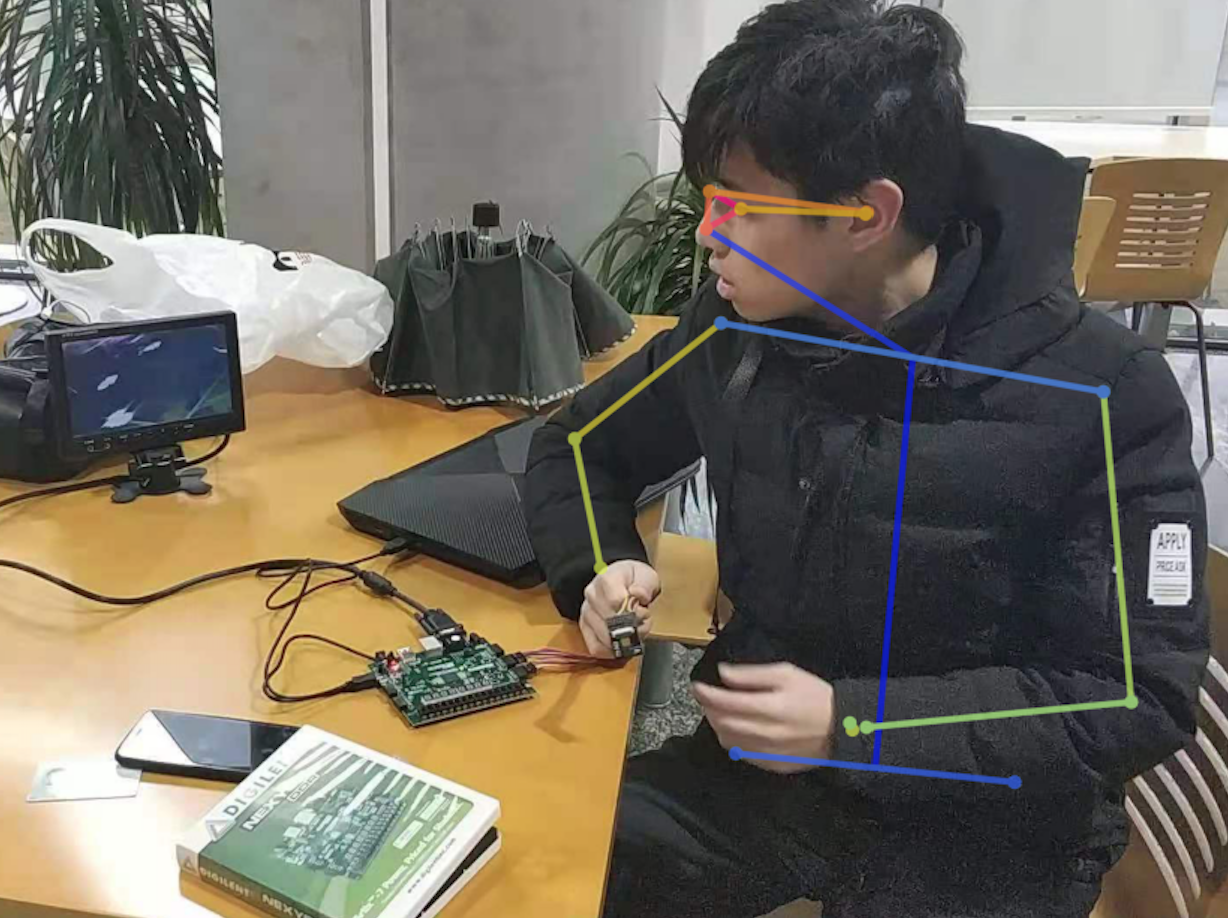
\includegraphics[width=\linewidth]{figures/pose.png}
    \end{minipage}\label{fig:pose}
    }
    %
    \caption{常见视频分析应用图解(图片提供者为中中同学)}\label{fig:cvexample}
    \centering
\end{figure}


\subsection{本文的工作}

本文的工作就是卷字数。

\subsection{文章结构}

采用递进式方法进行卷字数。

\newpage
\section{预备知识}\label{preliminaries}

\subsection{SOTA: 螺旋鲲鲲卷}

本节将介绍鲲鲲\cite{kun}是如何卷的。

\subsection{SOTA: 霹雳中中卷}

本节将介绍中中\cite{zhong}是如何卷的。

\newpage
\section{算法设计}\label{algorithm}

\subsection{伟伟卷卷法}

\subsubsection{电竞法}

每天12小时的英雄联盟游戏时间。

\subsubsection{追剧法}

每天再抽12小时看Netflix。

\newpage
\section{实验比较}\label{numerical experiments}

\subsection{内卷竞赛}

本节分别使用鲲鲲内卷法,中中内卷法,伟伟内卷法进行时间比较。在3天内,让实验组和对照组分别在3天内写论文。鲲鲲卷卷法3天写出了一篇CVPR,中中卷卷法3天写出了一篇AAAI,对照组三天写出了一份10页报告,而伟伟卷卷法3天从黄铜上分到了白银。

\newpage
\section{总结与未来工作展望}\label{conclusion}

写下你的未来工作展望。

\newpage

\addcontentsline{toc}{section}{参考文献}
\bibliography{note}

\newpage
\section*{谢\ 辞}
\addcontentsline{toc}{section}{谢辞}

本节通常用于感谢在研究过程中给予帮助和支持的人们,例如指导老师、实验室同学、朋友和家人等。

在谢辞中,需要真诚地表达感谢之情,回顾一下在研究过程中所受到的帮助和支持,并提到他们的具体贡献和重要性。同时,也可以简要说明一下自己在研究过程中的收获和体会,表达对他们的感激之情和祝福。

最后,需要注意不要出现太多的感情用词,语言简洁明了,表达真诚和诚恳即可。

谢谢支持本项目的所有朋友们。并且希望选用该模板的朋友们都能顺利通过查重与答辩。


\end{document}
